\documentclass{2wn20summary}

\usepackage{pgfplots}
\usepgfplotslibrary{fillbetween}

\begin{document}
	\maketitle
	\thispagestyle{empty}
	\newpage
	
	\section{Inleiding}
	
	Mocht je foutjes/opmerkingen/verbeteringen vinden, we zien ze graag op de \href{https://github.com/PHPirates/2WN20-summary/issues}{issue tracker}.
	
	Het boek waar naar verwezen wordt is \textbf{Numerical Methods for Ordinary Differential Equations}, \textit{C.~Vuik, F.J. Vermolen, M.B. van Gijzen, M.J. Vuik}.

	\section{College 1}
	\subsection{Floats}
		\indx{Floats} zijn van de vorm $\pm (0.d_1 d_2 d_3 \dots d_n)\beta^e = \pm  (d_1 \beta^{e-1}+d_2 \beta^{e-2}+\dots + d_n \beta^{e-n})$ met $e \in [L,U], \linebreak L<~0, U>~0$ de exponent, $\beta$ de basis (voor computers $2$), $(0.d_1 d_2 d_3 \dots d_n)$ de \indx{mantisse}. Vaak geldt $\abs{L},\abs{U} \in [100,10000]$. Verder geldt $ 0 < d_1 < \beta $.
		
		\begin{define}
		Voor $n$ zijn in principe twee mogelijkheden, $n=24$ met $0<d_i<\beta, i=2,3,\dotsc ,n$ heet \indx{single precision}, $n=53$ met $0 \le d_i < \beta$ heet \indx{double precision}. 
		\end{define}
		
		\begin{define}
			\[
				\abs{\fl(x)-x} \le \frac{1}{2} \beta^{e-n} \text{ heet een \indx{absolute rounding error},}
			\]
			\[
				\epsilon = \frac{\fl(x) - x}{x} \implies \fl(x) = x(1 + \epsilon) \text{ heet \indx{relative rounding error},}
			\]
			\[ 
				\abs{\epsilon} = \frac{\abs{\fl (x) - x}}{\abs{x}} \leq \beta^{1-n} \text{ heet \indx{machine precision}.}
			\]
		\end{define}
		
	\subsection{Rekenen met floats (ten opzichte van rekenen met de exacte waarde)}
		\begin{define}
			Rekenen met floats gaat als volgt, $ \fl (\fl (x) \circ \fl (y)) $ waar $ \circ \in \{+,-,\times, \div\} $. We bekijken het verschil met de exacte waarde. 
			\begin{align*}
				\abs{ x \circ y - \fl (\fl (x) \circ \fl (y)) } &= \abs{ x \circ y - \fl (x) \circ \fl (y) + \fl (x) \circ \fl (y) - \fl (\fl (x) \circ \fl (y))} \\
				&\leq \abs{x \circ y - \fl (x) \circ \fl (y)} + \abs{\fl (x) \circ \fl (y) - \fl (\fl (x) \circ \fl (y))}.
			\end{align*}
			$ \abs{x \circ y - \fl (x) \circ \fl (y)} $ heet de \indx{transmission error} of \indx{doorwerkingsfout}. Deze heeft te maken met de afronding.
			
			$  \abs{\fl (x) \circ \fl (y) - \fl (\fl (x) \circ \fl (y))} $ heet de \indx{calculation error} of \indx{bewerkingsfout}.
		\end{define}
		
		\begin{note}
			Voor optellen $ (+) $ en aftrekken $ (-) $ is de absolute error relevant. Voor vermenigvuldigen $ (\times) $ en delen $ (\div) $ is de relative error relevant.
		\end{note}
		
	\subsection{\indx{Landau orde symbool}}
		\begin{define}
			$ f(x) = \bigO (g(x)) $ for $ x \to 0 $. Then there exist an $ M > 0, r>0 $ such that
			\[ 
				\forall_{x \in [-r,r]}:\abs{f(x)} \leq M \abs{g(x)}\,.
			\]
		\end{define}
		
		\begin{theorem}
			Stel $ f(x) = \bigO(x^p), g(x) = \bigO(x^q) $ met $ p>0, q>0 $. Dan geldt het volgende:
			\begin{enumerate}[(i)]
				\item $ f(x) = \bigO(x^s) \qquad 0 \leq s < p $
				\item $ \alpha f(x) + \beta g(x) = \bigO (x^{\min (p,q)}) $
				\item $ f(x)g(x) = \bigO(x^{p+q}) $
				\item $ \frac{f(x)}{x^s} = \bigO(x^{p-s}) \qquad 0 \leq s < p $.
			\end{enumerate}
		\end{theorem}
		
	\subsection{Taylorpolynoom}
		\begin{theorem}
			Stel $ f(x) \in C^{(n+1)}[a,b] $ met $ x \in (a,b) $ en $ c \in (a,b) $.	Dan is er een $ \xi $ tussen $x$ en $c$ zodanig dat
			\begin{align*}
				f(x) &= P_n(x) + R_n(x) \\ 
				&= f(c) + (x-c)f'(c) + \frac{(x-c)^2}{2!}f''(c) + \dots + \frac{(x-c)^n}{n!}f^n(c) + \frac{(x-c)^{n+1}}{(n+1)!}f^{(n+1)}(\xi).
			\end{align*}
			We noemen dan $ \frac{(x-c)^{n+1}}{(n+1)!}f^{(n+1)}(\xi) $ de \indx{foutterm}\index{error Taylor polynomial}.
		\end{theorem}

	\newpage
	\section{College 2}
	\subsection{Interpolatie}
		\begin{define}
			Stel $ f(x) \in C[a,b] $ en $ x_0, x_1 \in (a,b) $, dan geldt voor het \indx{interpolatiepolynoom} $ p(x) $ dat
			\begin{align*}
				p(x) &= f(x_0) + \frac{f(x_1) - f(x_0)}{x_1 - x_0} \\
					&= \frac{x-x_1}{x_0-x_1}f(x_0) + \frac{x-x_0}{x_1-x_0}f(x_1)\,.
			\end{align*}
			
			\begin{tikzpicture}
			\begin{axis}[
				ylabel=$f(x)$,
				ytick={2,4},
				yticklabels={$f(x_0)$,$f(x_1)$},
				xlabel={$x$},
				xtick={0,2,4,8},
				xticklabels={$a$,$x_0$,$x_1$,$b$}
			]
				\addplot[samples=200, red, domain=0:8]{3 + sin(deg(2*x)} node[below] {$f(x)$};
				% p(x):
				\addplot[samples=20, dashed, domain=0:2]{x};
				\addplot[samples=20, domain=2:4]{x} node[above,pos=1]{$p(x)$};
				\addplot[samples=20, dashed, domain=4:8]{x};
			\end{axis}
			\end{tikzpicture}
		\end{define}
		
		\paragraph{Analyse fout in $ p(x) $}
			\begin{theorem}
				Voor het verschil tussen $ f(x) $ en $ p(x) $ geldt het volgende:
				\[ 
					f(x) - p(x) = \frac{1}{2} (x-x_0)(x-x_1)f''(\xi) \qquad \xi \in (x_0,x,x_1)\,.
				\]
				Oftewel, $ \xi $ ligt in het open interval opgespannen door de uitersten van $ x_0, x, x_1 $ (we sluiten extrapolatie niet uit).
			\end{theorem}
			
			Voor een verstoorde $f$ schrijven we $\hat{f}$. Definieer nu $ \epsilon_0 > 0 $ en $ \epsilon_1 > 0 $ de storing op $ f(x_0) $ en $ f(x_1) $ door $ \abs{\hat{f}(x_0) - f(x_0)}\leq \epsilon_0 $ en $ \abs{\hat{f}(x_1) - f(x_1)} \leq \epsilon_1 $, waarbij $ f(x_0) $ en $ f(x_1) $ de exacte waardes zijn. Definieer vervolgens $ \epsilon = \max (\epsilon_0, \epsilon_1) $. Dan volgt voor de verstoring op $ p(x) $
			\[ 
				\abs{\hat{p}(x) - p(x)} \leq \abs{\frac{x-x_1}{x_0-x_1}}\epsilon_0 + \abs{\frac{x-x_0}{x_1-x_0}}\epsilon_1 = \frac{\abs{x-x_1}\epsilon_0+\abs{x-x_0}\epsilon_1}{x_1-x_0} \leq \frac{\abs{x-x_1}+\abs{x-x_0}}{x_1-x_0}\epsilon\,.
			\]
			Voor interpolatie is $ \abs{\hat{p}(x) - p(x)} \leq \epsilon$. Voor extrapolatie is dit $ \abs{\hat{p}(x) - p(x)} \leq (1 + 2 \frac{\abs{x-x_1}}{x_1-x_0})\epsilon $. We zien dus dat interpolatie veilig is en de fout beperkt blijft. 
		
		\subsection{Lagrange interpolatie}
			\begin{define}
				Bij \indx{Lagrange interpolatie} is het interval waarover ge\"interpoleerd wordt verdeeld in $n$ deelintervallen. Het interpolatiepolynoom $ L_n(x) $ is gegeven door
				\[ 
					L_n(x) = \sum_{k=0}^n L_{kn} (x) f(x_k), \qquad \text{ met $ L_{kn}$ de \indx{Lagrange co\"efficienten}. }
				\]
				Deze Lagrange co\"efficienten worden gegeven door
				\[ 
					L_{kn}(x) = \frac{(x-x_0)(x-x_1)\dotsm(x-x_{k-1})(x-x_{k+1})\dotsm(x-x_n)}{(x_k-x_0)(x_k-x_1)\dotsm(x_k-x_{k-1})(x_k-x_{k+1})\dotsm(x_k-x_n)}\,.
				\]
				Er volgt 
				$\begin{cases}
					L_{kn}(x_j) = 1 & k = j \\
					L_{kn}(x_j) \neq 1 & k \neq j
				\end{cases} \ $.
				
				Voor de fout (die wordt veroorzaakt door verstoringen in functiewaarden) geldt nu
				\[ 
					\abs{\hat{L}_n(x)-L_n(x)} \leq \sum_{k=0}^n \abs{L_{kn}(x)} \epsilon, \qquad \text{met } \epsilon = \max (\epsilon_0, \epsilon_1, \dotsc, \epsilon_n).
				\]
			\end{define}
			\begin{note}
				Lineaire interpolatie is Lagrange interpolatie voor $n=1$, oftewel \indx{eerste orde Lagrange interpolatie}.
			\end{note}
	
		%TODO stuk tussen Lagrange and Cubic splines...
		\subsection{Kubische splines (\indx{Cubic splines})}
			
			\begin{define}
				\indx{Stuksgewijze interpolatie} houdt in dat het interval waarvoor we een interpolatiepolynoom willen beschrijven wordt opgedeeld in kleinere deelintervallen en we vervolgens voor elk deelinterval een interpolatiepolynoom beschrijven. Het gevolg hiervan is dat we knikken krijgen.
			\end{define}
			
			\begin{define}
				%TODO plaatje
				We willen een interpolatiepolynoom beschrijven voor de functie $f(x)$ op het interval $(a,b)$. We delen het interval $(a,b)$ op in $n$ deelintervallen, $(x_0,x_1), \dotsc, (x_{n-1}, x_n)$. Op elk deelinterval beschrijven we een \indx{kubische spline}, $S_0, S_1, \dotsc, S_{n-1}$. 
				\[ 
					S_j(x) = a_j(x-x_j)^3 + b_j(x-x_j)^2 + c_j(x-x_j) + d_j, \qquad \text{met } j = 0, \dotsc, n-1\,.
				\]
				We hebben nu $n-1$ vergelijkingen, en dus $4n$ onbekenden. Om deze onbekenden te vinden, stellen we een aantal eisen/voorwaarden aan $ S_j(x) $.
				\begin{align*}
					\textbf{Functiewaarden: } &S_j(x_j) = f(x_j) \\
						&S_{n-1}(x_n) = f(x_n) \\
					\textbf{Aansluitvoorwaarden: } &S_j(x_{j+1}) = S_{j+1} (x_{j+1}) \\
						&S_j '(x_{j+1}) = S_{j+1} ' (x_{j+1}) \\
						&S_j '' (x_{j+1}) = S_{j+1} '' (x_{j+1}) \\
					\textbf{"Randvoorwaarden": } &S_0 ''(x_0) = 0 \\
						&S_{n-1} '' (x_n) = 0
				\end{align*}
			\end{define}
			
		\newpage
		\section{College 3}
		\subsection{\indx{Eindige differenties} (benaderen van afgeleiden)}
		
			\begin{tikzpicture}
			\begin{axis}[
			axis lines = left,
			xmin=-2, xmax=2, ymin=-3.5, ymax=0.5,
			ylabel=$f(x)$,
			ytick={2,4},
			yticklabels={$f(x_0)$,$f(x_1)$},
			xlabel={$x$},
			xtick={0,0.5},
			xticklabels={$x$, $x+h$}
			]
				\addplot[samples=200]{-x^2};
				\addplot[dashed] coordinates {(0,-3.5) (0,0)};
				\addplot[dashed] coordinates {(0.5,-3.5) (0.5,-0.25)};
				\addplot[] coordinates {(-0.75,0) (0.75,0)} node[above]{$f'(x)$};
			\end{axis}
			\end{tikzpicture}
			
			\begin{define}
				De afgeleide van $ f(x) $ is gedefinieerd als $ f'(x) = \lim_{h \to 0} \frac{f(x+h)-f(x)}{(x+h) - x} = \lim_{h \to 0} \frac{f(x+h)-f(x)}{h} $. Voor een voorwaartse benadering van de afgeleide definieren we \index{Qv@$Q_v(x,h)$}
				\[ 
					Q_v(x,h) = \frac{f(x+h)-f(x)}{h}, \qquad \text{met $h$ eindig} \,.
				\]
				Het verschil tussen deze benadering en de werkelijke afgeleide noemen we de \indx{afbreekfout}. Deze is gegeven door
				\[ 
					f'(x) - Q_v(x,h) = f'(x) -  \frac{f(x+h)-f(x)}{h} = - \frac{h}{2} f ''(\xi), \qquad \text{voor } f \in C[x,x+h], \xi \in (x,x+h)\,.
				\]
				
				Verder bekijken we de achterwaartse benadering \index{Qa@$Q_a(x,h)$}
				\[ 
					 Q_a(x,h) = \frac{f(x)-f(x-h)}{h} \qquad \text{met $h$ eindig} ,
				\]
				met bijbehorende afbreekfout $ f'(x) - Q_a(x,h) = \frac{h}{2} f ''(\eta) $, $\eta \in (x-h,h)$.
				
				Tenslotte bekijken we de centrale benadering, wat het gemiddelde is van de voor- en achterwaartse benaderingen. \index{Qc@$Q_c(x,h)$}
				\[ 
					Q_c(x,h) = \frac{1}{2} (Q_v(x,h) + Q_a(x,h)) = \frac{f(x+h)-f(x-h)}{2h}\,.
				\]
				De afbreekfout die volgt is $ f'(x) - Q_c(x,h) = \frac{-h^2}{6} f'''(\xi), \xi \in (x-h, x+h) $.
			\end{define}

			\begin{define}
				De \indx{afrondfout} \index{rounding error} voor $ Q_c(x,h) $ is gegeven door
				\[
					\abs{Q_c(x,h) - \hat{Q}_c(x,h)} = \abs{\frac{f(x+h)-f(x-h)}{2h}- \frac{\hat{f}(x+h) - \hat{f}(x-h)}{2h}} \leq \frac{\epsilon_1 + \epsilon_2}{2h} \leq \frac{\epsilon}{h}, \qquad \epsilon = \max (\epsilon_1, \epsilon_2)\,.
				\]
				De \indx{totale fout} is de afbreekfout plus de afrondfout. Voor $ Q_c(x,h) $ is dit dus
				\[
					\abs{\frac{-h^2}{6}f'''(\xi)} + \frac{\epsilon}{h} \leq \frac{h^2}{6}\max\abs{f'''(\xi)}+ \frac{\epsilon}{h}\,.
				\]
				Verder geldt dat de afrondfout $ = \bigO(h^{-1}) $ en de afbreekfout $ = \bigO(h^2) $. Dit betekent dat als $h$ groter wordt de afrondfout kleiner wordt, maar de afbreekfout groter. Er is dus een optimale $h$ waarvoor de totale fout minimaal is.
			\end{define}

		\subsection{Richardson extrapolatie}
			\indx{Richardson extrapolatie} is een praktische manier om afbreekfouten te schatten zonder gebruik te maken van afgeleiden van $ f(x) $. Zie boek 3.7 page 33.



	\newpage
	\section{College 4}
		We bekijken differentiaalvergelijkingen van de vorm
		\[
			y' = \frac{\d y}{\d t} = f(t,y) \,, y = y(t) \,, \text{ beginvoorwaarde } y(t_0) = y_0 \,,
		 \]
		 met $f(t,y),t_0,y_0$ gegeven.

		 \begin{voorbeeld}

		 	$y'=\lambda y,\ y(t_0)=y(0)=y_0$ is nog exact op te lossen, en heeft als oplossing $y=y_0 e^{\lambda t}$. We kiezen hier voor het gemak $\lambda <0$, omdat we daardoor fysische stabiliteit garanderen.
		 \end{voorbeeld}
		 \begin{define}
		 	$y'=f(t,y)$ is \indx{goed gesteld} \index{well posed}indien er een unieke oplossing $y=y(t)$ bestaat die continu afhangt van $y(t_0)=y_0$.

		 	Een karakterisering is
		 	\[
			 	\abs{\frac{\partial f(t,y)}{\partial y}} \le L \in \reals \ \forall{t,y} \text{ in het te beschouwen rekendomein (t-waarden)}.
		 	 \]
		 	 Dit kennen we ook als \indx{Lipschitz-continu\"iteit}.
		 \end{define}

		 \begin{define}
		 	We noemen $y'=f(t,y)$ de \indx{differentiaalvorm}, $y(t_0) = y_0$. Dit is om te vormen in $y(t) = y_0 + \int_{t_0}^t f(\tau,y) \d \tau$, de \indx{integraalvorm} (impliciet).
		 \end{define}

		 \subsection{Numerieke methoden voor differentiaalvergelijkingen}
		 \subsubsection{\indx{Voorwaarts Euler} (instabiel)}
			 We benaderen $y(t) \approx y_0 + h f(t_0,y_0)$ met $h=t-t_0$, stukgewijs. Dus $y(t_1) \approx y_0 + h f(t_0,y_0) = w_1$, $y(t_1)$ is de exacte oplossing en $w_1$ de numerieke, en $w_2 = w_1 + h f(t_1,w_1)$, enzovoort.

			 Algemener geldt dan $w_{j+1}+h f(t_j,w_j)$ met $h=t_{j+1}-t_j$, dit is dus een expliciete formule.
			 
			 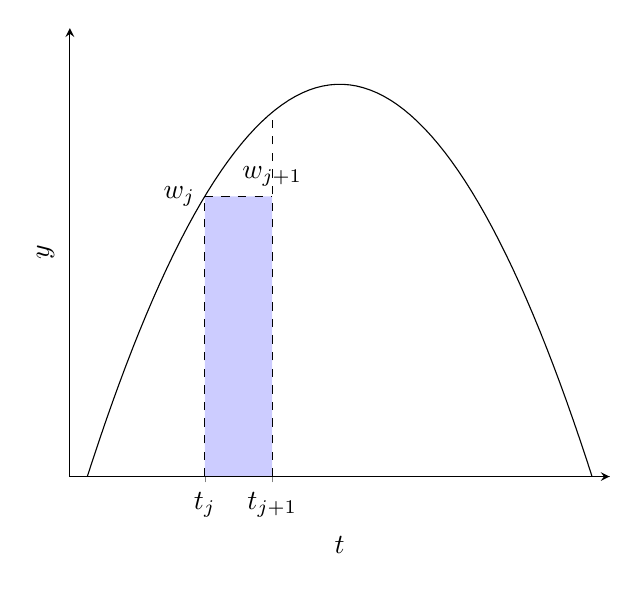
\begin{tikzpicture}
			 \begin{axis}[
					 axis lines = left,
					 xmin=-2, xmax=2, ymin=-3.5, ymax=0.5,
					 ylabel=$y$,
					 ytick=\empty,
					 xlabel={$t$},
					 xtick={-1,-0.5},
					 xticklabels={$t_j$, $t_{j+1}$}
				 ]
				 \addplot[samples=200]{-x^2};
				 \addplot[name path=C] 	coordinates {(-2,-3.5) (2,-3.5)};
				 \addplot[dashed] 		coordinates {(-1,-3.5) (-1,-1)} node[above,left]{$w_j$};
				 \addplot[dashed] 		coordinates {(-0.5,-3.5) (-0.5,-0.25)};
				 \addplot[dashed, name path=D] coordinates {(-1,-1) (-0.5,-1)} node[above]{$w_{j+1}$};
				 \addplot[blue!20] fill between[of=C and D,soft clip={domain=-1:-0.5}];
			 \end{axis}
			 \end{tikzpicture}
			 
		\subsubsection{\indx{Achterwaarts Euler} (iets stabieler)}
			Hier geldt de impliciete formule
			\[
				w_{j+1} = w_j + h f(t_{j+1},w_{j+1}) \,.
			 \]
			 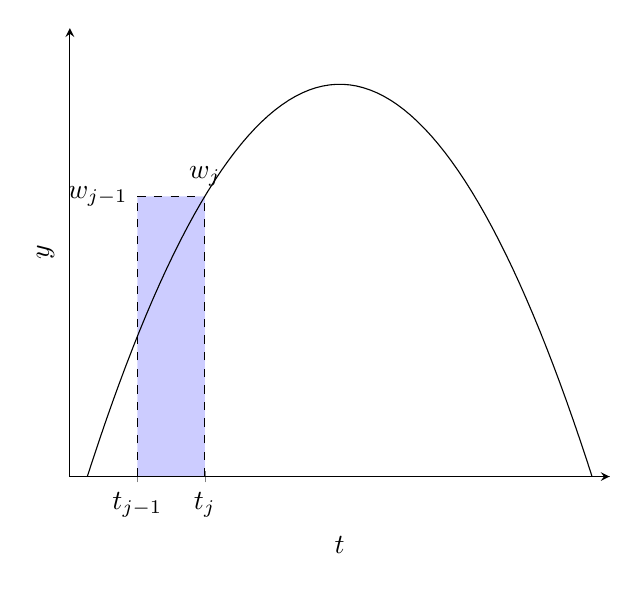
\begin{tikzpicture}
			 \begin{axis}[
					 axis lines = left,
					 xmin=-2, xmax=2, ymin=-3.5, ymax=0.5,
					 ylabel=$y$,
					 ytick=\empty,
					 xlabel={$t$},
					 xtick={-1.5,-1},
					 xticklabels={$t_{j-1}$, $t_j$}
				 ]
				 \addplot[samples=200]{-x^2};
				 \addplot[name path=C] 	coordinates {(-2,-3.5) (2,-3.5)};
				 \addplot[dashed] 		coordinates {(-1,-3.5) (-1,-1)} node[above]{$w_j$};
				 \addplot[dashed] 		coordinates {(-1.5,-3.5) (-1.5,-1)}node[above,left]{$w_{j-1}$};
				 \addplot[dashed, name path=D] coordinates {(-1.5,-1) (-1,-1)};
				 \addplot[blue!20] fill between[of=C and D,soft clip={domain=-1.5:-1}];
			 \end{axis}
			 \end{tikzpicture}
			 
		\subsubsection{\indx{Trapeziumregel}}
			Weer een impliciete formule
			\[
				w_{j+1} = w_j + \frac{h}{2} ( f(t_j,w_j) + f(t_{j+1},w_{j+1})) \,.
			 \]
		\subsubsection{\indx{Modified Euler}}
			Dit is een expliciete vorm van de trapeziumregel. Het doet eerst een voorspelling met voorwaarts Euler, $\overline w_{j+1} = w_j + h f(t_j,w_j)$. Dan volgt een correctiestap $w_{j+1} = w_j + \frac{h}{2} (f(t_j,w_j) + f(t_{j+1},\overline w_{j+1}))$ .

		\subsection{Versterkingsfactoren van de methoden}
			Toegepast op $y'=\lambda y,\ y(t_0) = y_0$.
			\paragraph{Voorwaarts Euler}
				\begin{define}
				Er geldt dus $w_{j+1} = w_j + h \lambda w_j = (1+\lambda h) w_j$, waarbij de \indx{versterkingsfactor} $Q(\lambda,h) = 1+\lambda h$.
				\end{define}
			Je kunt nagaan dat de andere versterkingsfactoren respectievelijk
			\[
				\frac{1}{1-\lambda h},\ \frac{1+\frac{h}{2}\lambda}{1-\frac{h}{2}\lambda},\ 1+h\lambda + \frac{1}{2} (h\lambda)^2
				\]
				zijn.

		\subsection{Verstoringen in beginwaarden}
			\begin{define}
			Gegeven de vergelijkingen
			\begin{align}
				y'=\lambda y,\ & y(t_0) = y_0 \\
				\hat y' = \lambda \hat y,\ & \hat y (t_0) = \hat y_0
			\end{align}
			met $\epsilon_0 = \hat y_0 - y_0$ als verstoring in beginvoorwaarde, dan volgt uit $(2)-(1)$
			\[
				\hat y' - y'=\lambda (\hat y-y) \implies \epsilon'=\lambda \epsilon,\ \epsilon(t_0) = \epsilon_0
			 \]
			 waarbij $\epsilon'=\lambda \epsilon$ de \indx{evolutievergelijking} voor de verstoring is.
			 \end{define}

			 \paragraph{\indx{Stabiliteitseisen} }
			 Er zijn twee mogelijkheden, de 'gewone' stabiliteitseis dat $ \abs{\epsilon(t)} $ eindig is voor alle $t$, of de \indx{absolute stabiliteitseis} dat $ \lim_{t\to \infty} \abs{\epsilon(t)} = 0 $. Let op, dit gaat over wiskundige stabiliteit, fysische stabiliteit was al afgedwongen door $\lambda <0$ te nemen.

			 Je kunt nagaan dat voor Voorwaarts Euler de (gewone) numerieke stabiliteit geldt bij $ \abs{1+\lambda h} \le 1 $ en dus $ h \le \frac{2}{\abs{\lambda}}. $

			 Evenzo volgt uit verdere stabiliteitsanalyses dat Achterwaarts Euler en de Trapeziumregel onvoorwaardelijk stabiel zijn, maar Modified Euler ook als voorwaarde $ h \le \frac{2}{\abs{\lambda}} $ heeft.
			 \begin{theorem}In het algemeen geldt dat expliciete numerieke methodes voor gewone differentiaalvergelijkingen, zoals Voorwaarts en Modified Euler, voorwaardelijk stabiel zijn, en impliciete methodes zoals Achterwaarts Euler en de Trapeziumregel onvoorwaardelijk stabiel zijn.
			 	\end{theorem}

			 	\paragraph{\indx{Numerieke stabiliteitsanalyse} voor willekeurige $ f(t,y) $}

			 	Dit doen we door lokaal te lineariseren.
			 	\[
				 	f(t,y) = f(t_j,y_j) + (t-t_j) \frac{\partial f}{\partial t}(t_j,y_j) + (y-y_j)\frac{\partial f}{\partial y}(t_j,y_j)
			 	 \]
			 	 Dit is makkelijker te onthouden door te zien dat dit gaat als bij $y'=\lambda y +g(t)$ met $\lambda =\frac{\partial f}{\partial y}(t_j,y_j)$.
			 	 \begin{voorbeeld}

			 	 	Zij $ y'=-10y^2 $ niet lineair, dan
			 	 	\[
				 	 	\frac{\partial f}{\partial y}(t_j,y_j) = -20 y_j = "\lambda"
			 	 	 \] en stel we gebruiken Voorwaarts Euler dan moet gelden $ h \le \frac{2}{\abs{\lambda}} $. Oftewel \[
				 	 	 h \le \frac{2}{\abs{\lambda}}= \frac{2}{20\abs{y_j}} = \frac{1}{10\abs{y_j}}.
			 	 	  \]
		 	 	  \end{voorbeeld}

		\subsection{\indx{Local truncation error} }
			\begin{define}
			De \indx{lokale afbreekfout} $\tau_{j+1} \coloneqq \frac{y_{j+1}-z_{j+1}}{h}$ met $z_{j+1}$ de numerieke oplossing uitgaande van de exacte oplossing op $t_j:\ y_j$.
			\end{define}

			\begin{voorbeeld}
				Zij $y'=\lambda y$.
				Voor Modified Euler geldt $ z_{j+1} = (1+\lambda h + \frac{1}{2} (\lambda h)^2)y_j $ en dus (met behulp van een Taylorexpansie van $y_{j+1}=e^{\lambda h}$)
				\[
					\frac{(1+\lambda h + \frac{1}{2}(\lambda h)^2 + \frac{1}{3}(\lambda h)^3+\dotsm) - Z_{j+1}}{h} = O(h^2).
				 \]
			\end{voorbeeld}

			\begin{define}

				$e_{j+1}=w_{j+1}-y_{j+1}$ is de \indx{lokale discretisatiefout} (de fout in de oplossing).
			\end{define}
			$\tau_{j+1}$ is een maat voor de nauwkeurigheid waarmee $\int_t^{t_{j+1}} f(\tau,y) \d \tau$ word ge\"evalueerd.

			%todo wat wordt hiermee bedoeld?:
			\[
				y'=f(t,y) \to y(t_j) = y(t_j) + \int_t^{t_{j+1}} f(\tau,y) \d \tau \text{ (exact)}
			 \] %etc

	\newpage
	\section{College 5}
		\subsection{Convergentie}
		Stel $ y' = f(t,y) $, met $f$ niet lineair. We weten de lokale afbreekfout $ \tau_{j+1} = \frac{y_{j+1}-z_{j+1}}{h} $. We noemen $ \abs{e_{j+1}} $ de \indx{globale discretisatiefout}, deze willen we zo klein mogelijk. We defini\"eren $ e_j=y_j-w_j $. We stellen de volgende convergentie-eis.
		\[ 
			\lim_{h \downarrow 0} e_j = 0 \,.
		\]
		%TODO plaatje Thomas
		Oftewel, we eisen $ \abs{e_j} = \bigO(h^p) $, met $ p>0 $.
		
		We beschouwen de testvergelijking $ y' = \lambda y $, met $ \lambda < 0 $. We hebben hier voor $ e_j $
		\begin{align*}
			e_j = y_j - w_j &= y_j - z_j + (z_j - w_j) \\
				&= h\tau_j + Q(\lambda h) (y_{j-1}-w_{j-1}) \\
				&= h\tau_j + Q(\lambda h) (h\tau_{j-1} + Q(\lambda h)e_{j-2})\,.
		\end{align*}
		We zien dat we hier te maken hebben met recursie. We kunnen deze recursie voortzetten tot $ e_0 $. $ e_0$ is gedefinieerd als $ e_0 = y_0 - w_0 = 0 $. Hieruit volgt
		\[ 
			e_j = \sum_{l=0}^{j-1} (Q(\lambda h))^l h \tau_{j-l}\,.
		\]
		
		\subsubsection{Numerieke stabiliteit}
			We weten 
			\[ 
				\abs{e_j} \le \sum_{l=0}^{j-1} \abs{Q(\lambda h)}^l h \abs{\tau_{j-l}}\,. 
			\]
			Voor numerieke stabiliteit eisen we $ \abs{Q(\lambda h) \le 1} $. Dit geeft 
			\[ 
				\abs{e_j} \le \sum_{l=0}^{j-1} h \abs{\tau_j-l} \le M \tau_{\max}\,, \qquad \text{met $M$ eindig, } M \ge jh, \tau_{\max} = \max \abs{\tau_{j-l}}\,.
			\]
		\subsection{Consistentie}
			We stellen de volgende consistentie-eis.
			\[ 
				\lim_{h\downarrow 0} \tau_j = 0\,, \qquad \text{met }\tau_j = \bigO(h^p), p>0\,.
			\]
			\begin{voorbeeld}
				Voor voorwaarts Euler geldt $ \tau_j = \bigO(h) $, dus voorwaarts Euler is een consistente methode.
			\end{voorbeeld}
			
			\begin{theorem}[\indx{Lax equivalentiestelling}] 
				Indien een numerieke methode numeriek stabiel en consistent is, dan is deze methode ook convergent.
			\end{theorem}
			
			\begin{opm}
				Bij numerieke methoden met $ \tau_j = \bigO(h^p) $ en numerieke stabiliteit hebben we $ e_j = \bigO(h^p) $.
			\end{opm}
		
		\subsection{\`a la Richardson extrapolatie}
			Als de exacte oplossing ($ y(t_j,h) $) onbekend is, kunnen we $ p $ bepalen op een manier vergelijkbaar met Richardson extrapolatie. We gebruiken de volgende vergelijkingen.
			\begin{align}
				y(t_j,h) - w_j &= e_j = K_1 h^ p + K_2 h^ {p+1} + \dots \approx Kh^p\,, \qquad \text{met $K,p$ onbekend en constant.}\label{ala1} \\
				y(t_{2j}, \frac{h}{2}) - w_{2j} &= e_{2j} = K(\frac{h}{2})^p \,. \label{ala2} \\
				y(t_{4j}, \frac{h}{4}) - w_{4j} &= e_{4j} = K(\frac{h}{4})^p \,. \label{ala4} 
			\end{align}
			We gebruiken deze vergelijkingen om $p$ te kunnen berekenenen.
			\begin{align*}
				\frac{(\ref{ala1})-(\ref{ala2})}{(\ref{ala2})-(\ref{ala4})} &= \frac{w_{2j}-w_j}{w_{4j}-w_{2j}} = \frac{h^p (1-(\frac{1}{2})^p)}{h^p ((\frac{1}{2})^p- (\frac{1}{4})^p)} =\frac{1-(\frac{1}{2})^p}{(\frac{1}{2})^p- (\frac{1}{4})^p} = 2^p\,. \\
				p &= \log_2\left( \frac{1-(\frac{1}{2})^p}{(\frac{1}{2})^p- (\frac{1}{4})^p} \right)\,.
			\end{align*}
			
			\subsection{Stelsel differentiaal vergelijkingen}
				\begin{voorbeeld}[Prooidier-roofdier probleem, Gekoppels stelsel diff verg]
					Stel $ y_1(t) = \#$konijnen, $\linebreak y_2(t) = \# $vossen. Verder geldt
					\begin{align*}
						\frac{\d}{\d t} y_1 &= c_1 y_1 - c_2 y_1 y_2 \qquad \text{(voortplanting konijnen - consumptie door vossen)} \\
						\frac{\d}{\d t} y_2 &= c_3 y_ 1 y_2 - c_4 y_2 \qquad \text{(voortplanting vossen - verhongering vossen)}
					\end{align*}
					met beginvoorwaarden $ y_1(t_0), y_2(t_0) $ gegeven. 
					Dit kunnen we ook schrijven met vectoren. 
					\[ 
						\frac{\d \y}{\d t} = \f (\y)\,, \qquad \f = \begin{pmatrix}
						c_1 y_1 - c_2 y_1 y_2 \\ c_3 y_ 1 y_2 - c_4 y_2
						\end{pmatrix}, \y = \begin{pmatrix}
							y_1 \\ y_2
						\end{pmatrix}.
					\]
				\end{voorbeeld}
				\begin{voorbeeld}[Mathematische slinger]
					Tweede orde differentiaal vergelijking.
					\[ 
					ml\frac{\d^2 \phi}{\d t^2} = -mg\sin \phi \implies \phi '' = \frac{-q}{l} \sin \phi \,.
					\]
					We defini\"eren $ y_1 = \phi, y_2 = \frac{\d \phi}{\d t} $. We krijgen nu de volgende differentiaal vergelijking, waar we $2$ beginvoorwaarden voor nodig hebben, namelijk $ y_1(t_0), \frac{d y_1}{d t}(t_0) $.
					\[ 
						\frac{\d}{\d t}\y = \begin{pmatrix}
							y_2 \\ \frac{-g}{l} \sin y_1
						\end{pmatrix}.
					\]
				\end{voorbeeld}
				
				\begin{opm}
					De numerieke methoden die we eerder hebben gezien (VE, AE, Trapezium regel, ME) zijn hier hetzelfde als voor scalaire vergelijkingen, maar dan met vectoren.
				\end{opm}
				
				We beschouwen de test vergelijking $ y'= \lambda y, \lambda < 0 $. In vectoren hebben we dan $ \y ' = A \y + \g (t), \y(t)= \y_0 $, met $A$ een matrix die in principe vol is. Voor verstoorde $\y$ hebben we $ \hat{\y}' = A\hat{\y} + \g(t) $. Voor de afrondfout $\epsilon$ hebben we $ \vec{epsilon}\,' = A\vec{\epsilon} $, met $ \vec{\epsilon}_0 (t_0) = \hat{\y_0}-\y $. Dit stelsel is \indx{gekoppeld}.
				
				\textbf{Truc:} voer in $ \vec{\epsilon} = S\vec{\eta} $, met $\eta$ de getransformeerde verstoringen, en $S$ een matrix met als kolommen de eigenvectoren van $A$. Nu hebben we $ S\vec{\eta} \,' = AS\vec{\eta} \implies \vec{\eta}\,' = S^{-1}AS\vec{\eta}$. Dit stelsel is \indx{ontkoppeld}.
				
				\textbf{Eis voor fysische stabiliteit van het stelsel}
				\[ 
					\lambda_i \in \complex \: \text{Re}(\lambda_i) \le 0\, \forall_i\,.
				\]
				
				\paragraph{Stabiliteitsanalyse van voorwaarts Euler.} Er geldt $ \vec{\epsilon_{j+1}} = A \vec{\epsilon_j} + hA\vec{\epsilon_j} = (I + hA)\vec{\epsilon_j} $. Dit is een gekoppeld stelsen, en dit stelsel is numeriek stabiel als $ ||I+hA||\le 1 $. We passen de truc toe en krijgen $ \vec{\eta_{j+1}} = S^{-1} (I+hA)S\vec{\eta_j} = (I+h\Lambda)\vec{\eta_j} $. Dit stelsel is ontkoppeld, en numeriek stabiel voor $ \abs{1+h\lambda_i} \le 1 $. Het stabiliteitsgebied voor voorwaarts Euler is de cirkel rond $ -1+0i $ met straal $1$. Deze methode is ongeschikt voor zuiver imaginaire $i$.
				
				Voor achterwaarts Euler is het stabiliteitsgebied alles buiten de cirkel rond $ 1+0i $ met straal $1$. Deze methode is dus veel geschikter voor zuiver imaginaire $i$.
				
	\newpage
	\section{College 6}
	
	\subsection{Belang van hogere orde nauwkeurigheid}
	
		Als we Voorwaarts Euler ($O(h)$) bekijken, $w_{j+1} = w_j + hf(t_j,w_j)$, zien we dat dit \'e\'en $f$-evaluatie bevat. Modified Euler ($O(h^2)$), verkort te schrijven als
		\[ 
			w_{j+1} = w_j + \frac{h}{2} (f(t_j,w_j) + f(t_{j+1},w_j + hf(t_j,w_j)))
		 \]
		 bevat echter effectief twee $f$-evaluaties. Dit kunnen we ook in een tabel weergeven aan de hand van $e_n$, de globale discretisatiefout.
		 
		 \[ 
			 \begin{array}{c|cc|cc|c}
				 & \text {Voorwaarts Euler} & & \text {Modified Euler} & & \\
				 e_n & \text {stapgrootte} & \text {\#f-evaluaties} & \text {stapgrootte} & \text {\#f-evaluaties} & \text {beste} \\
				 \hline
				 \alpha & h &n &h &2n & \text {VE} \\
				 \alpha /4 & h/4 & 4n & h/2 & 4n & - \\
				 \alpha /16 & h/16 & 16n & h/4 & 8n & \text {ME} \\
				 \alpha /64 & h/64 & 64n & h/8 & 16n & \text {ME}
			 \end{array}
		  \]
		  
		  We zien hier dat een methode van hogere orde nauwkeurigheid \textbf{niet} per s\'e beter % hij zei nauwkeuriger maar betwijfel of dat zo is
		   is, maar zich anders gedraagt bij een kleiner wordende $h$.
		  
	\subsection{\indx{Stijve differentiaalvergelijkingen}}
		Gegeven de vergelijking $\y'=\f (t,\y )$, bepalend voor fysische stabiliteit zijn de eigenwaarden $\lambda_i$ van $\frac{\partial \f  }{\partial \y }$. Bij Voorwaarts Euler hebben we een beperkt stabiliteitsgebied, namelijk de cirkel met straal 1 en middelpunt (-1,0) $(1+h \mu_i)^2 +h \nu_i^2 \le 1 \forall_i$ waarbij $h\mu_i$ op de 'x-as' en $h \nu_i$ op de 'y-as' staat. Daarom kan het voorkomen dat er \'e\'en eigenwaarde heel ver weg ligt waardoor je $h$ heel erg klein moet nemen om alle eigenwaarden in de cirkel te krijgen. Dit is een typisch stijf probleem.		  
		
		Bij impliciete methoden zoals Achterwaarts Euler en de Trapeziumregel is het stabiliteitsgebied zo groot dat je geen kleine $h$ hoeft te nemen.
		
	\subsection{\indx{Method of manufactured solutions}}
	
		We gaan hier uit van een scalaire, lineaire, inhomogene differentiaalvergelijking $y'=\lambda y + g(t)$.
		
		We maken een differentiaalvergelijking door uit te gaan van een oplossing $y(t) = C e^{\lambda t} +F(t)$, met $C$ een constante en $F(t)$ een particuliere oplossing. Hieruit volgt $y'(t) = C\lambda e^{\lambda t} + F'(t)$.
		
		Als we dit terugsubstitueren krgijen we
		\begin{align*}
			C \lambda e^{\lambda t} + F'(t) &= \lambda (C e^{\lambda t} +F(t)) + g(t) \\
			g(t) &= F'(t) - \lambda F(t)
		\end{align*}
		oftewel de inhomogene term in termen van de particuliere oplossing.
		
		\begin{voorbeeld}
			Stel $C=-1$ en $\lambda = -1000$, dan kunnen we zien dat bij Voorwaarts Euler (en expliciete methoden in het algemeen) een $h\le \frac{2}{|\lambda|} = \frac{1}{500}$ nodig is. Dat is vervelend omdat zo'n kleine $h$ alleen dicht bij de oorsprong nodig is en daarna niet meer omdat de $e$-macht dan 'uitgedoofd' is. Impliciete methoden zijn onvoorwaardelijk stabiel dus daar zouden we de $h$ kunnen aanpassen aan wat nodig is (eerst klein, dan groter).
		\end{voorbeeld}
		
			We zien ook dat de versterkingsfactor van Achterwaarts Euler $Q(\lambda h)=\frac{1}{1-\lambda h}$ naar nul nadert als $\lambda h \to - \infty$, dus dit is stabiel (verstoringen doven snel uit). Echter bij de Trapeziumregel nadert de versterkingsfactor $Q(\lambda h)=\frac{1+\lambda h/2}{1-\lambda h/2}$ naar -1 als $\lambda h \to - \infty$, en als je dan in het begin een te grote $h$ hebt gekozen dan dempt de fout niet snel uit en krijg je grote oscillaties.
			
		\subsection{\indx{Runge-Kutta methoden}} 
			Dit is een klasse van \indx{\'e\'enstapsmethoden}, dat wil zeggen dat deze van $t_j$ naar $t_{j+1}$ gaan. Bijvoorbeeld Voorwaarts Euler is RK1, Modified Euler is RK2. Modified Euler, normaal geschreven als
			\begin{align*}
				\overline w_{j+1} &= w_j + h f(t_j,w_j) \\
				w_{j+1} &= w_j + \frac{h}{2} (f(t_j,w_j) + f(t_{j+1},\overline w_{j+1}))
			\end{align*}
			is op de Runge-Kutta manier te schrijven als
			\begin{align*}
				k_1 &= hf(t_j,w_j) \\
				k_2 &= hf(t_{j+1},w_j + k_1) \\
				w_{j+1} &= w_j + \frac{1}{2}(k_1 + k_2) \,,
			\end{align*}
			waar $k_1$ en $k_2$ hulpgrootheden noemen. Hierdoor is ook makkelijk te zien dat dit inderdaad slechts twee effectieve $f$-evaluaties zijn.
			
		\subsubsection{\indx{RK4 (standaard)}}
			Dit is een $4^e$ orde nauwkeurige methode ook voor niet-lineaire problemen, als volgt definieerd:
			\begin{align*}
				k_1 &= hf(t_j,w_j) \\
				k_2 &= h f(t_j+\frac{1}{2} h,w_j + \frac{1}{2}k_1) \\
				k_3 &= hf (t_j+\frac{1}{2}h,w_j + \frac{1}{2}k_2) \\
				k_4 &= hf(t_j + h,w_j + k_3) \\
				w_{j+1} &= w_j + \frac{1}{6} (k_1 + 2k_2 + 2k_3 + k_4)\quad \text {\indx{Simpsonregel}}
			\end{align*}
			De Simpsonregel is een integratieregel voor $\int_{t_j}^{t_{j+1}} f(\tau,y) \d \tau$ net als Voorwaarts Euler of de Trapeziumregel.
			
		\subsection{Meerstapsmethoden}
			We beschouwen $y'=f(t,y)$ met de Trapeziumregel, $w_{j+1} = w_j + \frac{h}{2} (f(t_j,w_j) + f(t_{j+1}, w_{j+1}))$. Nu gaan we $f$ extrapoleren zodat $f(t_{j+1}, w_{j+1})$ vervangend wordt door $2f(t_j,w_j)-f(t_{j-1},w_{j-1})$. Dit is een $O(h^2)$ extrapolatie vanuit $t_{j-1},t_j$.
			
			Een andere mogelijkheid is \indx{Adams-Bashforth}, met
			\[ 
				w_{j+1} = w_j + \frac{3h}{2} f(t_j,w_j) - \frac{h}{2} f(t_{j-1},w_{j-1}) \,.
			 \]
			 \begin{opm}
			 	Door mogelijk grote extrapolatie kunnen grote fouten ontstaan
			 \end{opm}
			 \begin{opm}
				 Deze methoden zijn niet zelfstartend, dus er zijn ook andere methoden nodig
			 \end{opm}
			 
			 Dor een analyse van Adams-Bashforth te doen blijkt dat (voor een testvergelijking $y'=\lambda y$) de stabiliteitseis voor twee mogelijke versterkingsfactoren $\abs{Q_{1,2}} \le 1$. Door consistentie te testen volgt ook de orde, en misschien ook wel convergentie met de Lax-stelling.
		                  

	\section{College 7}

	\section{College 8}
	
	\section{College 9}
	
	\section{College 10}


	\phantomsection
	\newpage
	\addcontentsline{toc}{chapter}{Index} 
	\printindex
	
	
\end{document} 
